\chapter{Background}\label{background}
\section{Neural Networks}
A neural network is a machine learning tool ideal for conducting supervised learning. As a relatively recent field, the application of neural networks has rapidly extended across many domains, such as  facial recognition at Facebook \cite{deepface}, translation for Microsoft \cite{translation}, spam filters for Google's Gmail \cite{gmail} and more. As such, it continues to be a hot topic in today's world of research.

\subsection{The Neuron}
The \textit{neuron} is the basic computational unit of a neural network. A \textit{layer} is comprised of one or more neurons. The computation performed by a neuron is shown below.
\begin{align}
\text{net} &= \mathbf{w \cdot x} + b\label{eq2.1}\\
y &= f(\text{net})
\end{align}
The \textit{fan-in} to a neuron is the amount of elements in the input vector $\mathbf{x} = x_1, x_2, \ldots, x_n$. For each element, there is a corresponding parameter referred to as a \textit{weight}. The weights of a neuron form the weight vector $\mathbf{w}$. The neuron also has an offset $b$ which helps with normalization. The neuron's net is first computed as shown in equation \ref{eq2.1}, and then the output, or activation, is computed according to the neuron's activation function. This is shown visually in figure \ref{neuron}.
\begin{figure}
	\centering
	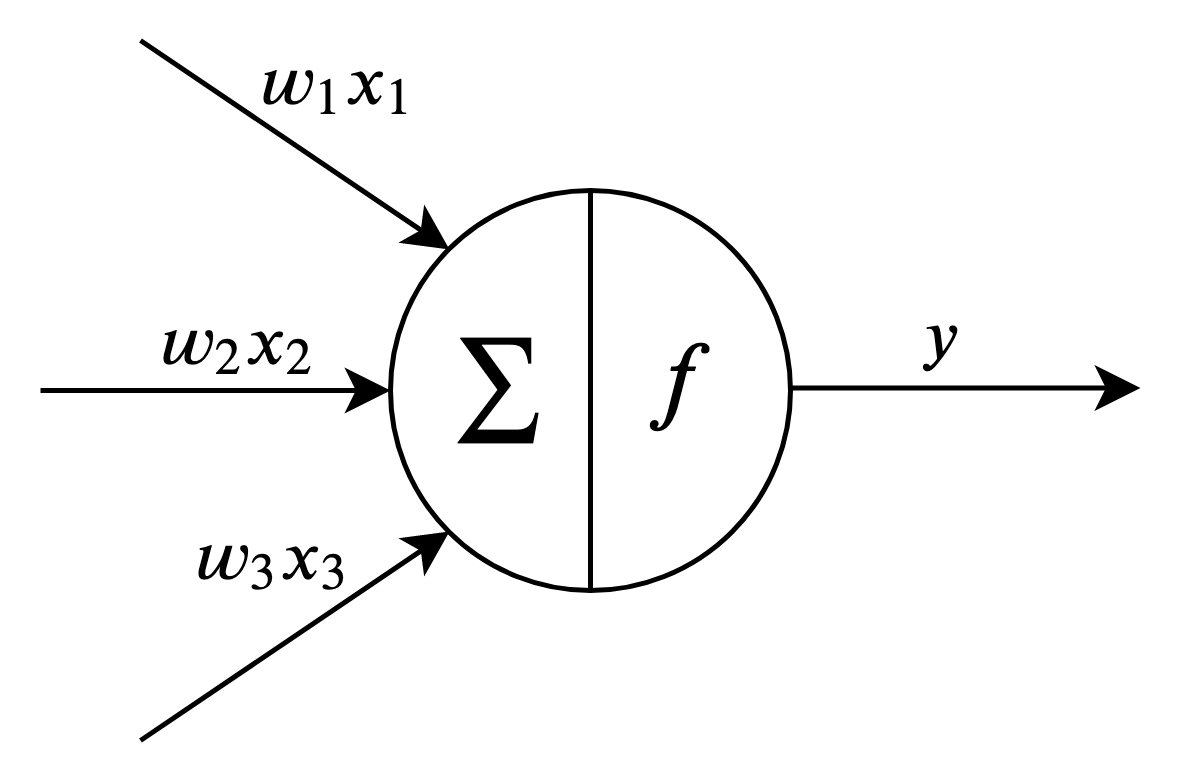
\includegraphics[width=2in]{figures/neuron}
	\caption{A neuron with 3 inputs; bias term omitted for simplicity.}\label{neuron}
\end{figure}

\paragraph{Weight Initialization}
Proper weight initialization is paramount to successfully training a neural network. Firstly, weights cannot be all initialized to 0, for this will result in the same gradient for all weights, and thus all weights will be updated in the same manner. This would effectively mean that the network would become a function of a singular weight.

The most na\"ive way to initialize weights would to assign each weight a random value between some range. In most cases, this is good enough for the network to converge to a relatively optimal solution so long as the range is not to extreme. 
\todo[inline]{He initialization with proper paper cite}


\subsection{Fully-Connected Layers}
A fully-connected layer is a vector of neurons. All neurons in a fully-connected layer receive the same input vector. This vector is the previous layer's output. A fully-connected layer with 3 neurons receiving input from an input layer is shown in figure \ref{fully-connected}. The output is a vector comprising of the outputs of each neuron. Each neuron output is calculated using the $M$-sized input vector as shown in equation \ref{n-act} and added to output vector $\mathbf{y}$.
\begin{align}
y_i &= f_{\text{act}}\left( b + \sum_{j=1}^{M}(w_jx_j) \right) \label{n-act} \\
\mathbf{y} &= \left\{ y_1, y_2, \ldots, y_n \right\} 
\end{align}

\begin{figure}
	\centering
	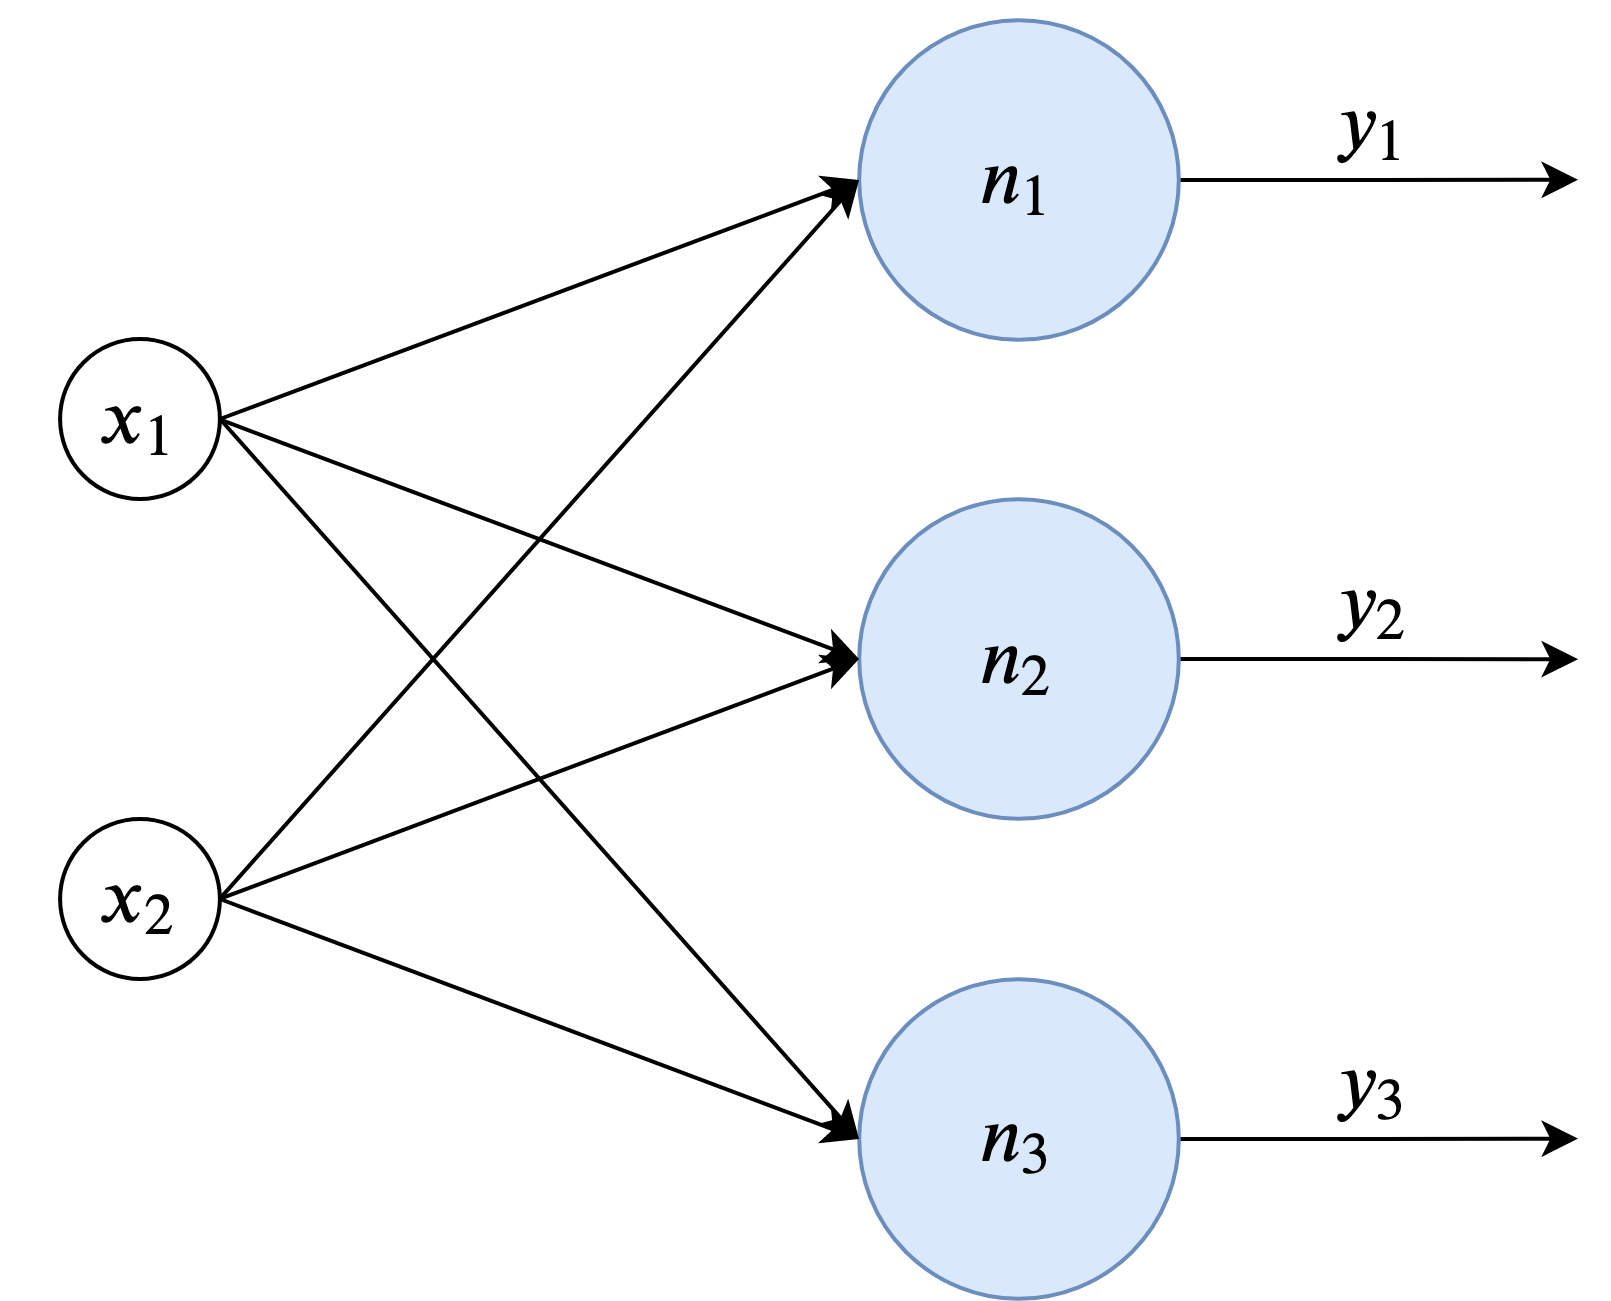
\includegraphics[width=3in]{figures/fully-connected}
	\caption{A fully-connected layer with 3 neurons, each receiving an input vector of size 2 from the input layer.}\label{fully-connected}
\end{figure}

\subsection{Activation Functions}
Without activation functions, the neural network would simply devolve to a linear classifier. Activation functions provide neural networks with the non-linearity to solve complex classification problems. Two of the most common activation functions are the rectified linear unit (ReLU) and the softmax function. These are the two activation functions that were chosen to be used in the software and hardware models of this thesis.

\paragraph{ReLU}
ReLU is a powerful activation function that has found widespread use due to its mathematical simplicity. The ReLU function is shown in equation \ref{relu-func}.
\begin{align}
y = \max(0, x) \label{relu-func}
\end{align}
Notably, the ReLU function is much easier to compute compare to the sigmoid or hyperbolic tangent functions, which both use the exponential function. The ReLU function also quite frequently performs just as well if not better compared to other activation functions. One of the reasons is because it does not suffer as much from the vanishing gradient problem \cite{pmlr-v15-glorot11a}. The vanishing gradient problem is encountered during training using backpropagation, which uses the chain rule from calculus, briefly covered in section \ref{backprop}. Since gradients will always be less than 1 for most loss functions, the gradients become geometrically smaller with each layer. Since ReLU only saturates in one direction, ReLU networks will be more sparse, in the sense that many of the neurons will have an output of 0. 

ReLU-based neural networks also tend to reach convergence quicker than neural networks using the sigmoid or the hyperbolic tangent functions. It also results in a sparsely activated network, in that since the neuron output is 0 if the net is negative, that many neurons in the network will have an output of 0. This is also similar to how biological neurons also follow a sparse firing model, and has shown to be effective \cite{pmlr-v15-glorot11a}. 

Conversely, since active neurons in ReLU network are sparse, this brings rise to another potential problem, the ``Dying ReLU Problem.'' This problem occurs when the sparsity increases to the point where a large majority of the neurons in the network become inactive during training and ultimately never become active again. Fortunately, this problem can be ameliorated with proper weight initialization \cite{Lu2019DyingRA}.

\paragraph{Softmax}
The softmax function converts a vector of logits to a vector of probabilities. It has seen widespread use in neural networks that are used to predict the class of an input. The softmax function is shown in equation \ref{sm-func}.
\begin{align}
\sigma(\mathbf{x})_i = \frac{e^{x_i}}{\Sigma_{j=1}^C e^{x_j}} \label{sm-func}
\end{align}
In this function, $x_i$ is the net of neuron $i$ from the last layer. Each neuron in the last layer represents a class, so the size of the last layer is equivalent to the number of classes, $C$. 


\subsection{Cross-Entropy Loss}
Cross-entropy loss is a probabilistic loss function and as such, is frequently paired with the softmax activation function. This allows for the probabilities output from the softmax function to be used as inputs for calculating the cross-entropy loss. Cross-entropy loss is computed using probabilities and is shown in equation \ref{cel-eq}.
\begin{align}
\mathcal{L}(\mathbf{x}) = \sum_{i=1}^{N} q(x_i)\log(p(x_i))\label{cel-eq}
\end{align}
In this function, $q(x_i)$ is the true probability of $x$ belonging to class $i$, therefore, $q(x_i) = 1$ when $x$ is of class $i$ and $0$ otherwise; $p(x_i)$ is equal to the predicted probability.

\subsection{Backpropagation}\label{backprop}
Backpropagation is a method in which the weights of a network can be trained on a dataset by propagating the loss from the output layer backward through the network. It utilizes the chain rule from calculus to propagate the loss.


\subsection{Hyperparameters}
\paragraph{Learning Rate}
\paragraph{Batch Size}
\paragraph{Momentum}
\paragraph{Training Epochs}


\section{Deep-Learning Frameworks}
Deep-learning has come into the spotlight in the past few years and as such, many popular and robust frameworks have been developed. Some of the most popular frameworks are TensorFlow which is developed by Google, and PyTorch which is developed by Facebook. Other popular frameworks include Keras and Caffe. These frameworks are generally relatively simple to use while delivering high performance. 


\subsection{PyTorch}
For this thesis, PyTorch has been chosen as the framework to construct a model against which to benchmark my results. PyTorch offers a simplistic interface to build highly customizable neural networks. In addition, it also has support for GPU-training, thus both CPU and GPU benchmarks can be obtained.

\section{Related Work}